\documentclass[10pt]{article}
\usepackage[a4paper, margin=2cm]{geometry}
%\usepackage{fullpage}
\usepackage[T1]{fontenc}
\usepackage[utf8]{inputenc}
\usepackage{graphicx}
\usepackage{mathpazo}
\pagenumbering{arabic}
\usepackage{siunitx}
\usepackage{amsmath}
\usepackage{mathtools} % Para poder usar "\Aboxed"
\usepackage{cancel} % Para usar "\cancel", de https://tex.stackexchange.com/questions/537955/how-do-cross-out-text-in-math-mode
\usepackage{multicol}
\usepackage[spanish]{babel}
\usepackage{steinmetz}
\DeclareSIUnit\voltampere{VA}
\DeclareSIUnit\var{VA_r}
\setlength\parindent{0pt} % no indent

% Numbering pages on the right footer:
% (https://tex.stackexchange.com/questions/153167/how-to-set-page-number-at-right-footer)
\usepackage{fancyhdr}
% Turn on the style
\pagestyle{fancy}
\fancyhf{} % sets both header and footer to nothing
\renewcommand{\headrulewidth}{0pt} % To remove the top horizontal line created by default by "fancyhdr", from here: https://tex.stackexchange.com/questions/13896/how-to-remove-the-top-horizontal-bar-in-fancyhdr
% Set the right side of the footer to be the page number
\fancyfoot[R]{\thepage}


\usepackage{minibox} % Para poder partir el texto en 2 líneas usando "underbrace" u "overbrace", info aquí: https://tex.stackexchange.com/questions/8680/how-can-i-insert-a-newline-in-a-framebox


\usepackage{xparse} % For "overbrace/underbrace but with an arrow instead", from https://tex.stackexchange.com/questions/8720/overbrace-underbrace-but-with-an-arrow-instead

% Para poner flechas sobre los signos de igual, de aquí: https://tex.stackexchange.com/questions/8720/overbrace-underbrace-but-with-an-arrow-instead
\NewDocumentCommand{\overarrow}{O{=} O{\uparrow} m}{%
  \overset{\makebox[0pt]{\begin{tabular}{@{}c@{}}#3\\[0pt]\ensuremath{#2}\end{tabular}}}{#1}
}
\NewDocumentCommand{\underarrow}{O{=} O{\downarrow} m}{%
  \underset{\makebox[0pt]{\begin{tabular}{@{}c@{}}\ensuremath{#2}\\[0pt]#3\end{tabular}}}{#1}
}





\begin{document}

\large{\textbf{Enunciado}}:

\vspace{3mm}
Un generador de corriente continua alimenta dos cargas. La primera de estas cargas está situada a \qty{2100}{\meter} del generador, tiene una resistencia de \qty{215}{\ohm} y rendimiento unidad. La segunda carga está situada \qty{270}{\meter} después de la primera, tiene una potencia de \qty{4662}{\watt}, un rendimiento del 75\% y una tensión aplicada de \qty{420}{\volt}.

La línea es de cobre, de \qty{6}{\milli\meter\squared} de sección y con una resistividad de \qty{17.24}{\milli\ohm\milli\meter\squared\per\meter}.

\vspace{4mm}

Con esta información, se debe calcular:

\vspace{1mm}

\begin{enumerate}
    \item La tensión en bornes del generador
    \item La corriente entregada por el generador
    \item El rendimiento de la instalación
\end{enumerate}


\hrulefill

\vspace{5mm}
\textbf{Solución}:
\vspace{4mm}

Empezamos dibujando el esquema del circuito y organizando los datos disponibles:
\vspace{6mm}

\begin{minipage}{0.725\linewidth}
  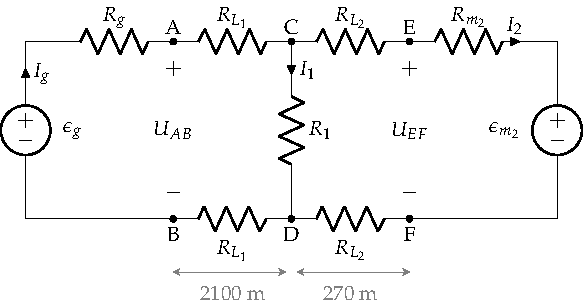
\includegraphics[scale=1.18]{../figs/circuito_ejercicio2_BT1.pdf}
\end{minipage}
\begin{minipage}{0.275\linewidth}

  \vspace{-5mm}
  \textbf{Datos}:
  
  \vspace{2mm}

  $l_1 = \qty{2100}{\meter}$\\
  $R_1 = \qty{215}{\ohm}$\\
  $\eta_1 = 100\%$\\
  $l_2 = \qty{270}{\meter}$\\
  $P_2 = \qty{4662}{\watt}$\\
  $\eta_2 = 75\%$\\
  $U_{EF} = \qty{420}{\volt}$\\
  $\rho_L = \qty{17.24}{\milli\ohm\milli\meter\squared\per\meter}$\\
  $S_L = \qty{6}{\milli\meter\squared}$
\end{minipage}

\vspace{6mm}

Unos apuntes sobre la información de que disponemos:
\begin{itemize}
    \item Dado que la primera de las cargas tiene rendimiento unidad, toda la potencia que recibe es potencia útil. Al tener esta carga una resistencia, para que pueda tener un rendimiento del 100\%, esta carga es necesariamente una \underline{resistencia pura}. Aunque típicamente usamos las resistencias para modelar pérdidas de energía por efecto Joule, en este caso la usamos para modelar calor como trabajo útil: esta carga podría representar, por ejemplo, un calefactor, cuya función es producir calor.
    \item Dado que la segunda carga tiene un rendimiento menor que la unidad, sabemos que no es un motor ideal, por lo que debemos incluir su resistencia interna, $R_{m_2}$.
    \item La potencia de la segunda carga, $P_2 = \qty{4662}{\watt}$, es su potencia útil.
    \item Dado que la tensión aplicada en la segunda carga es de \qty{420}{\volt}, esto implica que $U_{EF} = \qty{420}{\volt}$.
    \item Dado que hay dos nudos en el circuito (C y D), no hay una única corriente, sino tres distintas ($I_g, \, I_1, \, I_2$).
    \item En cuanto al generador: no tenemos información suficiente para saber si se trata de un generador ideal o real. Es recomendable asumir incialmente que es real, y si al resolver el problema llegamos a la conclusión de que $R_g=\qty{0}{\ohm}$, entonces se tratará de un generador ideal.
\end{itemize}


\vspace{6mm}

\underline{Apartado 1}

\vspace{4mm}

Debemos calcular la tensión en bornes del generador, es decir, la tensión a la salida del mismo, $U_{AB}$. 

Podemos hacerlo aplicando 2LK, una vez conozcamos $U_{AC}$ y $U_{CD}$ (dado que $U_{AC} = U_{DB}$). Para obtener estos valores:
\begin{itemize}
    \item Para calcular $U_{CD}$ es necesario conocer el valor de $R_{L_2}$ e $I_2$:

    Tenemos información sobre la carga 2: dado que conocemos su potencia útil y rendimiento, podemos calcular su potencia absorbida. Con la potencia absorbida, y usando la tensión a la entrada del motor, podemos calcular la corriente absorbida por este:
    
    \[
        \eta_m = \frac{P_{\textrm{útil}}}{P_{\textrm{absorbida}}} = \frac{\qty{4662}{\watt}}{U_{EF} \cdot I_2} = \frac{4662}{420\cdot I_2} = 0.75 \quad \rightarrow \quad I_2 = \qty{14.8}{\ampere}
    \]

    Una vez calculemos el valor de $R_{L_2}$, y conociendo ya la corriente $I_2$ que circula por ellas, podemos calcular la caída de tensión en la línea 2, y finalmente obtener $U_{CD}$:

    \[
        R_{L_2} = \rho \cdot \frac{l}{S} = {17.24 \cdot 10^{-3}} \cdot \frac{270}{6} = \qty{0.78}{\ohm}
    \]
    
    \vspace{-10mm}
    \[
        U_{CD} \overarrow[=][\downarrow]{\small 2LK}  U_{CE} + U_{EF} + U_{FD} = R_{L_2}\cdot I_2 + 420 + R_{L_2}\cdot I_2 = \qty{443.09}{\volt}
        % Flecha, sacada de aquí: https://tex.stackexchange.com/questions/8720/overbrace-underbrace-but-with-an-arrow-instead
    \]    

    \item Para calcular $U_{AC}$ necesitamos conocer tanto $R_{L_1}$ como $I_g$:

    \vspace{-7mm}
    \[
        I_1 = \frac{U_{CD}}{R_1} = \frac{443.09}{215} = \qty{2.06}{\ampere} \;\; \text{\small (ley de Ohm)} \quad \rightarrow \quad I_g \overarrow[=][\downarrow]{\small 1LK} I_1 + I_2 = 2.06 + 14.8 = \qty{16.86}{\ampere}
    \]
    \[
        R_{L_1} = \rho \cdot \frac{l}{S} = {17.24 \cdot 10^{-3}} \cdot \frac{2100}{6} = \qty{6.03}{\ohm}
    \]

    \vspace{-9mm}
    \[
        U_{AB} \overarrow[=][\downarrow]{\small 2LK}  U_{AC} + U_{CD} + U_{BD} = R_{L_1}\cdot I_g + 443.09 + R_{L_1}\cdot I_g = \boxed{ \qty{646.42}{\volt} }
        % Flecha, sacada de aquí: https://tex.stackexchange.com/questions/8720/overbrace-underbrace-but-with-an-arrow-instead
    \]
    
\end{itemize}


\vspace{4mm}

\underline{Apartado 2}

\vspace{4mm}

$I_g$ ya ha sido calculada en el apartado anterior, aplicando 1LK:

\[
    I_g = I_1 + I_2 = 2.06 + 14.8 = \boxed{ \qty{16.86}{\ampere} }
\]

\vspace{4mm}

\underline{Apartado 3}

\vspace{-1mm}

\[
    \eta_{\textrm{total}} = \frac{P_{\textrm{útil}}}{P_{\textrm{producida}}} = \frac{R_1\cdot I_1^2 + \epsilon_{m_2} \cdot I_2}{U_{AB} \cdot I_g} = \frac{215 \cdot 2.06^2 + \overbrace{\eta_2 \cdot U_{EF}}^{=0.75\cdot 420} \cdot 14.8}{646.42 \cdot 16.86} = \boxed{51.15\%}
\]

Nota: este rendimiento asume que el generador es ideal, dado que no conocemos su resistencia interna, y por lo tanto no podemos calcular sus pérdidas por efecto Joule.

Aunque el ejercicio ya está resuelto, vamos a calcular el rendimiento de cada elemento para entender mejor dónde ocurren las pérdidas en el circuito:

\begin{align*}
    \eta_{L_1} &= \frac{P_{\textrm{salida}}}{P_{\textrm{entrada}}} = \frac{U_{CD}\cdot \bcancel{I_g}}{U_{AB} \cdot \bcancel{I_g}} = \frac{443.09}{646.42} = 68.55\%\\[10pt]
    \eta_{R_1} &= 100\% \;\; \text{(dado en el enunciado)}\\[10pt]
    \eta_{L_2} &= \frac{P_{\textrm{salida}}}{P_{\textrm{entrada}}} = \frac{U_{EF}}{U_{CD}} = \frac{420}{443.09} = 94.79\%\\[10pt]
    \eta_{m_2} &= 75\% \;\; \text{(dado en el enunciado)}  
\end{align*}

Vemos que la línea 1 tiene unas pérdidas enormes, debidas a su gran longitud. Las pérdidas podrían reducirse eligiendo un conductor con una sección mayor, que haría disminuir la resistencia de la línea.


\end{document}
